%%%%%%%%%%%%%%%%%%%%%%%%%%%%%%%%%%%%%%%%%
% Beamer Presentation
% LaTeX Template
% Version 1.0 (10/11/12)
%
% This template has been downloaded from:
% http://www.LaTeXTemplates.com
%
% License:
% CC BY-NC-SA 3.0 (http://creativecommons.org/licenses/by-nc-sa/3.0/)
%
%%%%%%%%%%%%%%%%%%%%%%%%%%%%%%%%%%%%%%%%%

%----------------------------------------------------------------------------------------
%PACKAGES AND THEMES
%----------------------------------------------------------------------------------------

\documentclass{beamer}
\usepackage{listingsutf8}
\usepackage{listings}

\renewcommand{\figurename}{Figura}
\renewcommand{\tablename}{Tabla}
\renewcommand{\lstlistingname}{Recuadro}

\setbeamertemplate{caption}[numbered]

\colorlet{punct}{red!60!black}
\definecolor{background}{HTML}{EEEEEE}
\definecolor{delim}{RGB}{20,105,176}
\colorlet{numb}{magenta!60!black}


\lstdefinelanguage{json}{
    basicstyle=\normalfont\tiny,
    numbers=left,
    numberstyle=\tiny,
    stepnumber=1,
    numbersep=8pt,
    showstringspaces=false,
    breaklines=true,
    backgroundcolor=\color{background},
    literate=
     *{ticket}{{{\color{numb}ticket}}}{6}
      {content}{{{\color{numb}content}}}{7}
      {created\_at}{{{\color{numb}created\_at}}}{10}
      {address\_detail}{{{\color{numb}address\_detail}}}{14}
      {formatted_address}{{{\color{numb}formated\_address}}}{17}
      {zipcode}{{{\color{numb}zipcode}}}{7}
      {county}{{{\color{numb}county}}}{6}
      {long\_name}{{{\color{numb}long\_name}}}{9}
      {short\_name}{{{\color{numb}short\_name}}}{10}
      {state}{{{\color{numb}state}}}{6}
      {neighborhood}{{{\color{numb}neighborhood}}}{12}
      {group}{{{\color{numb}group}}}{5}
      {categories}{{{\color{numb}categories}}}{10}
      {:}{{{\color{punct}{:}}}}{1}
      {,}{{{\color{punct}{,}}}}{1}
      {\{}{{{\color{delim}{\{}}}}{1}
      {\}}{{{\color{delim}{\}}}}}{1}
      {[}{{{\color{delim}{[}}}}{1}
      {]}{{{\color{delim}{]}}}}{1},
}

\mode<presentation> {

% The Beamer class comes with a number of default slide themes
% which change the colors and layouts of slides. Below this is a list
% of all the themes, uncomment each in turn to see what they look like.

%\usetheme{default}
%\usetheme{AnnArbor}
%\usetheme{Antibes}
%\usetheme{Bergen}
%\usetheme{Berkeley}
%\usetheme{Berlin}
%\usetheme{Boadilla}
%\usetheme{CambridgeUS}
%\usetheme{Copenhagen}
%\usetheme{Darmstadt}
%\usetheme{Dresden}
%\usetheme{Frankfurt}
%\usetheme{Goettingen}
%\usetheme{Hannover}
%\usetheme{Ilmenau}
%\usetheme{JuanLesPins}
%\usetheme{Luebeck}
\usetheme{Madrid}
%\usetheme{Malmoe}
%\usetheme{Marburg}
%\usetheme{Montpellier}
%\usetheme{PaloAlto}
%\usetheme{Pittsburgh}
%\usetheme{Rochester}
%\usetheme{Singapore}
%\usetheme{Szeged}
%\usetheme{Warsaw}

% As well as themes, the Beamer class has a number of color themes
% for any slide theme. Uncomment each of these in turn to see how it
% changes the colors of your current slide theme.

%\usecolortheme{albatross}
%\usecolortheme{beaver}
%\usecolortheme{beetle}
%\usecolortheme{crane}
%\usecolortheme{dolphin}
%\usecolortheme{dove}
%\usecolortheme{fly}
%\usecolortheme{lily}
%\usecolortheme{orchid}
%\usecolortheme{rose}
%\usecolortheme{seagull}
%\usecolortheme{seahorse}
%\usecolortheme{whale}
%\usecolortheme{wolverine}

%\setbeamertemplate{footline} % To remove the footer line in all slides uncomment this line
%\setbeamertemplate{footline}[page number] % To replace the footer line in all slides with a simple slide count uncomment this line

%\setbeamertemplate{navigation symbols}{} % To remove the navigation symbols from the bottom of all slides uncomment this line
}

\usepackage{graphicx} % Allows including images
\usepackage{booktabs} % Allows the use of \toprule, \midrule and \bottomrule in tables
\lstset{inputencoding=utf8/latin1}

%----------------------------------------------------------------------------------------
%TITLE PAGE
%----------------------------------------------------------------------------------------

\title[]{Reconocimiento de Entidades para Filtrado de Duplicados} % The short title appears at the bottom of every slide, the full title is only on the title page

\author{Jorge Alberto Cordero Cruz} % Your name
\institute[FIME UANL]{
  Universidad Aut\'{o}noma de Nuevo Le\'{o}n\\~\\~\\
  
\includegraphics[scale=0.8]{imagenes/uanl.pdf} 
  }

\date{21 de enero del 2014} % Date, can be changed to a custom date

\begin{document}

\begin{frame}
  \titlepage % Print the title page as the first slide
\end{frame}

\begin{frame}%agenda de la presentacion
  \frametitle{Agenda}
  \begin{itemize}
  \item Motivaci\'{o}n para realizar detecci\'{o}n de documentos duplicados
  \item Hip\'{o}tesis
  \item Objetivos
  \item Reportes ciudadanos
  \item Sistema de detecci\'{o}n de duplicados
  \item Resultados
  \item Trabajos relacionados
  \item Estado actual de la tesis
  \end{itemize}
\end{frame}

\begin{frame}
  \frametitle{Motivaci\'{o}n para realizar detecci\'{o}n de documentos duplicados}
  Hoy en d\'{\i}a existe cierto nivel de presi\'{o}n para que los investigadores de las universidades produzcan art\'{\i}culos de investigaci\'{o}n. En ocasiones los investigadores plagian trabajos de otras personas. Por lo que una herramienta que permita detectar art\'{\i}culos cient\'{i}ficos duplicados ayudar\'{\i}a a bajar los niveles de plagio.\\
  \vspace{2mm}
  Todos los d\'{\i}as el \textcolor{blue}{Centro de Integraci\'{o}n Ciudadana (CIC)} recibe reportes (\textcolor{blue}{reportes ciudadanos}) de problemas de vialidad y tr\'{a}nsito, situaciones de riesgo, accidentes, etc. Varias personas pueden reportar un mismo suceso por lo que los reportes recibidos pueden ser duplicados. Una herramienta capaz de detectar reportes duplicados permitir\'{\i}a agilizar el proceso de respuesta del CIC ante los reportes.
\end{frame}

\begin{frame}
  \frametitle{Hip\'{o}tesis}
  \begin{itemize}
  \item Las t\'{e}cnicas de etiquetado y reconocimiento de entidades pueden ser utilizadas para generar una representaci\'{o}n estructurada a partir del contenido de diferentes tipos de documentos.\\
    \vspace{2mm}
  \item Una representaci\'{o}n estructurada permite utilizar t\'{e}cnicas de miner\'{\i}a de datos y aprendizaje m\'{a}quina sin tomar en cuenta los tipos de documentos con los que se trabaja.
    \vspace{2mm}
  \item Las t\'{e}cnicas de miner\'{\i}a de datos y aprendizaje m\'{a}quina pueden ser utilizadas para detectar documentos duplicados en un repositorio.
  \end{itemize}
\end{frame}
\begin{frame}
  \frametitle{Objetivos}
  El objetivo general consiste en detectar de manera autom\'{a}tica documentos duplicados en un repositorio de documentos.\\
  \vspace{2mm}
  Objetivos espec\'{\i}ficos:
   \begin{itemize}
  \item Extraer de diferentes tipos de documentos la informaci\'{o}n referente a:
    \begin{itemize}
      \item tiempos
      \item lugares
      \item informaci\'{o}n importante
      \item nombres de personas y nombres de organizaciones
    \end{itemize}
  \item Crear una representaciones estructuradas partir de la informaci\'{o}n extraida. 
  \item Detectar documentos duplicados aplicando algoritmos supervisados a las representaciones estructuradas.
  \end{itemize}
\end{frame}
%fin del protocolo de investigacion

\begin{frame}
  \frametitle{Reportes ciudadanos del CIC}
      En el trabajo desarrollado se utilizaron los reportes del CIC, los cuales fueron descargados desde la plataforma para desarrolladores CICMty-API en formato JSON. En la Tabla 1 se muestran las diferentes categor\'{i}as a las que pertenecen los reportes ciudadanos.
  \begin{table}\scriptsize
    \centering
    \begin{tabular}{|l|p{6cm}|}
      \hline
      \textbf{Grupos}&\textbf{Categor\'{\i}as}\\
      \hline
      Comunidad&Avisos, Evento p\'{u}blico, Observador ciudadano\\
      \hline
      Emergencia&Emergencias\\
      \hline
      Propuestas ciudadanas&Propuesta comunidad, Propuesta seguridad, Propuesta servicios p\'{u}blicos, Propuesta vialidad\\
      \hline
      Seguridad&Incendio, Robo, Situaci\'{o}n de riesgo\\
      \hline
      Servicios p\'{u}blicos&Alcantarillas, Alumbrado p\'{u}blico, Falta electricidad, Fuga, Otros, Parques descuidados, Recolecci\'{o}n de basura\\
      \hline
      Vialidad y tr\'{a}nsito&Accidente, Bache o v\'{\i}a da\~{n}ada, Obras y/o v\'{\i}a cerrada, Sem\'{a}foro descompuesto, Vialidad\\
      \hline
    \end{tabular}
    \caption{Grupos y categor\'{\i}as de grupo a las que puede pertenecer un reporte ciudadano}
  \end{table}      
\end{frame}

\begin{frame}
  \frametitle{Categor\'{i}as de reportes seleccionadas}
  Para este trabajo de tesis se seleccionaron reportes pertenecientes a las siguientes categor\'{\i}as: 
  \begin{itemize}
    \item \texttt{Accidente}
    \item \texttt{Alumbrado p\'{u}blico}
    \item \texttt{Sem\'{a}foro descompuesto}
    \item \texttt{Bache o v\'{\i}a da\~{n}ada}
    \item \texttt{Evento p\'{u}blico}
    \item \texttt{Alcantarillas}
    \item \texttt{Obras y/o v\'{\i}as cerradas}
    \item \texttt{Situaci\'{o}n de riesgo}
  \end{itemize}
\end{frame}


\begin{frame}
  \frametitle{Ejemplo de reportes duplicados}

  \begin{block}{Primer reporte}
    ACCIDENTE \colorbox{gray}{Unidad de la S.V.T.} de Monterrey acude \colorbox{gray}{al lugar}.\\
    En Lincoln y Aguaturma Paseo de Las Mitras \colorbox{green}{64118} Monterrey \colorbox{green}{NL} Mexico.\\
    2013-06-20 \colorbox{yellow}{09:59:28}
  \end{block}
  \vspace{5 mm}
  \begin{block}{Segundo reporte}
    ACCIDENTE \colorbox{gray}{transito} de Monterrey acude.\\
    En Aguaturma y Lincoln Paseo de Las Mitras Monterrey \colorbox{green}{Nuevo Leon} Mexico.\\
    2013-06-20 \colorbox{yellow}{09:49:46}
  \end{block}

\end{frame}

\begin{frame}
  \frametitle{Ejemplo de reportes no duplicados}
  
  \begin{block}{Primer reporte}
    ACCIDENTE \colorbox{gray}{Unidad de la S.V.T. de Monterrey acude al lugar}.\\
    En Lincoln y Aguaturma \colorbox{green}{Paseo} de Las Mitras \colorbox{green}{64118} Monterrey NL Mexico.\\
    2013-06-20 \colorbox{yellow}{09:59:28}
  \end{block}
  \vspace{5 mm}
  \begin{block}{Segundo reporte}
    ACCIDENTE \colorbox{gray}{choque de motos}.\\
    Avenida Lincoln y Aguaturma \colorbox{green}{P.} de Las Mitras Monterrey NL Mexico.\\
    2013-06-20 \colorbox{yellow}{15:59:28}
  \end{block}
\end{frame}

\begin{frame}
  \frametitle{Sistema propuesto}
  \begin{figure}
    \centering
    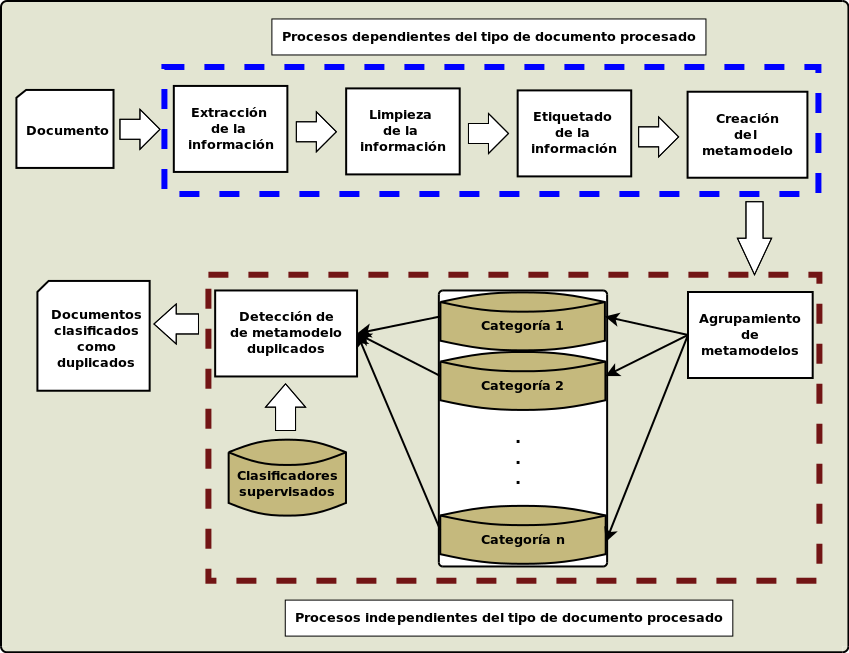
\includegraphics[width = 0.8\textwidth]{imagenes/diagrama2_tesis.png}
  \end{figure}
\end{frame}

\begin{frame}
  \frametitle{Reporte ciudadano en formato JSON}
  \begin{minipage}{0.1\linewidth}
  \end{minipage}
  \begin{center}
  \begin{minipage}{0.8\linewidth}
    \begin{figure}
      \lstinputlisting[frame=single, language=json]{sourceCode/reporteCIC.js}
    \end{figure}
  \end{minipage}
  \end{center}
  \begin{minipage}{0.1\linewidth}
  \end{minipage}
\end{frame}

\begin{frame}
  \frametitle{Extracci\'{o}n de la informaci\'{o}n}
  Los campos utilizados para extraer la informaci\'{o}n de los reportes son los siguientes:
  \begin{itemize}
  \item \texttt{'ticket'} (n\'{u}mero de ticket).
  \item \texttt{'content'} (contenido).
  \item \texttt{'created\_at'} (fecha de creaci\'{o}n).
  \item \texttt{'address\_detail':'formatted\_address'} (direcci\'{o}n con formato).
  \item \texttt{'categories'} (categor\'{\i}as).
  \end{itemize}
\end{frame}

\begin{frame}
  \frametitle{Limpieza de la informaci\'{o}n}
  Al texto extra\'{\i}do se aplican filtros para eliminar el ruido. Algunos de los filtros aplicados son los siguientes:
  \vspace{2 mm}
      
  \begin{itemize}
  \item Eliminaci\'{o}n de acentos
    \begin{itemize}
    \item \texttt{p\textcolor{blue}{\'{u}}blico} $\rightarrow$ \texttt{p\textcolor{blue}{u}blico}
    \end{itemize}
    \vspace{2 mm}

  \item Sustituci\'{o}n del punto (.) y dos puntos (:)
    \begin{itemize}
    \item \texttt{ave\textcolor{blue}{.}} $\rightarrow$ \texttt{ave\textcolor{blue}{\_dot\_}}
    \item \texttt{P\textcolor{blue}{.} Livas} $\rightarrow$ \texttt{P\textcolor{blue}{\_dot\_} Livas}
    \item \texttt{11\textcolor{blue}{:}16} $\rightarrow$ \texttt{11\textcolor{blue}{\_dot\_dot\_}16}
    \end{itemize}
    \vspace{2 mm}  

  \item Eliminaci\'{o}n de s\'{\i}mbolos
    \begin{itemize}
    \item \texttt{``@''}
    \item \texttt{``-''}
    \item \texttt{``*''}
    \end{itemize}
  \end{itemize}
\end{frame}

\begin{frame}
  \frametitle{Limpieza de la informaci\'{o}n}
  \begin{itemize}
  \item Eliminaci\'{o}n de palabras con expresiones regulares, por ejemplo hashtags:
    \begin{itemize}
    \item \texttt{r'\#[a-zA-Z\_0-9]+'} $\rightarrow$ \texttt{\#1Accidente}
    \end{itemize}
    \vspace{2 mm}

  \item Separaci\'{o}n de oraciones usando el punto final (.), por ejemplo: \textcolor{blue}{\texttt{``Choque en avenida Garza Sada. Enviar param\'{e}dicos.''}}
    \begin{itemize}
    \item Choque en avenida Garza Sada
    \item Enviar param\'{e}dicos
    \end{itemize}
    \vspace{2 mm}

  \item Sustituci\'{o}n de \_dot\_ y \_dot\_dot\_
    \begin{itemize}
    \item \texttt{ave\textcolor{blue}{\_dot\_}} $\rightarrow$ \texttt{ave\textcolor{blue}{.}} 
    \item  \texttt{P\textcolor{blue}{\_dot\_} Livas} $\rightarrow$ \texttt{P\textcolor{blue}{.} Livas}
    \item  \texttt{11\textcolor{blue}{\_dot\_dot\_}16} $\rightarrow$ \texttt{11\textcolor{blue}{:}16}
    \end{itemize}
    
  \end{itemize}
\end{frame}


\begin{frame}
 \frametitle{Ejemplo de texto original y texto limpio}
  
  \begin{block}{Texto original}
    \colorbox{green}{*ACCIDENTE*} en Ave. Garza Sada sin lesionados \colorbox{green}{param\'{e}dicos} acuden, 6:30 pm MTY NL \colorbox{yellow}{\#choquefuerte @cicmty via @colli03} gracias
  \end{block}
  
  \vspace{5 mm}
  
  \begin{block}{Texto limpio}
    \colorbox{green}{ACCIDENTE} en Ave. Garza Sada sin lesionados \colorbox{green}{paramedicos} acuden, 6:30 pm MTY NL gracias
  \end{block} 

\end{frame}

\begin{frame}
  \frametitle{Etiquetado de la informaci\'{o}n}
  El contenido de los textos limpios se etiqueta para identificar nombres de entidades correspondientes a \textcolor{blue}{\texttt{lugares}}, \textcolor{blue}{\texttt{tiempo}} e \textcolor{blue}{\texttt{informaci\'{o}n relevante}}. En este trabajo de tesis se uso un etiquetador muy sencillo basado en un \textcolor{blue}{Modelo Oculto de Markov}.
  \vspace{2 mm}\\
  Las etiquetas utilizadas en esta tesis fueron:
  \vspace{2 mm}
  \begin{itemize}
  \item \texttt{\textcolor{orange}{LOC}} para indicar un lugar
  \item \texttt{\textcolor{orange}{TIME}} para indicar tiempo
  \item \texttt{\textcolor{orange}{NAME}} para indicar nombres de personas
  \item \texttt{\textcolor{orange}{ORG}} para indicar nombres de organizaciones y/o empresas
  \item \texttt{\textcolor{orange}{TTERM}} para indicar informaci\'{o}n de un suceso reportado
  \item \texttt{\textcolor{orange}{O}} para indicar informaci\'{o}n irrelevante
  \end{itemize}
\end{frame}

\begin{frame}
  \frametitle{Ejemplo de reconocimiento de entidades}
  Del texto limpio \textcolor{blue}{\texttt{``ACCIDENTE en Ave. Garza Sada sin lesionados paramedicos acuden, 6:30 pm MTY NL gracias''}} se obtienen las siguientes entidades:\\
  \begin{itemize}
    \item \textcolor{orange}{\texttt{LOC}}: en, Ave., Garza, Sada y NL 
    \item \textcolor{orange}{\texttt{TIME}}: 6:30 y pm
    \item \textcolor{orange}{\texttt{TTERM}}: ACCIDENTE, sin, lesionados y paramedicos
    \item \textcolor{orange}{\texttt{ORG}}: gracias
  \end{itemize}
\end{frame}

\begin{frame}
  \frametitle{Creaci\'{o}n del metamodelo}
  Un \textcolor{blue}{metamodelo} es una representaci\'{o}n estructurada del contenido de un texto etiquetado.\\
  El \textcolor{blue}{metamodelo} permite aplicar los mismos algoritmos de detecci\'{o}n de duplicados a documentos de diferentes formatos (documentos PDF, p\'{a}ginas web, documentos JSON).\\
  
  \lstinputlisting[basicstyle=\footnotesize\ttfamily, language=XML, frame=single, caption=Metamodelo generado a partir de un texto etiquetado]{sourceCode/metamodeloCasoEstudio1.xml}
\end{frame}

\begin{frame}
  \frametitle{Creaci\'{o}n del metamodelo}
  Para cada tipo de documento que se procesa en el sistema se debe implementar el proceso de obtenci\'{o}n del metamodelo mostrado en la Figura 2.
  \begin{figure}
    \centering
    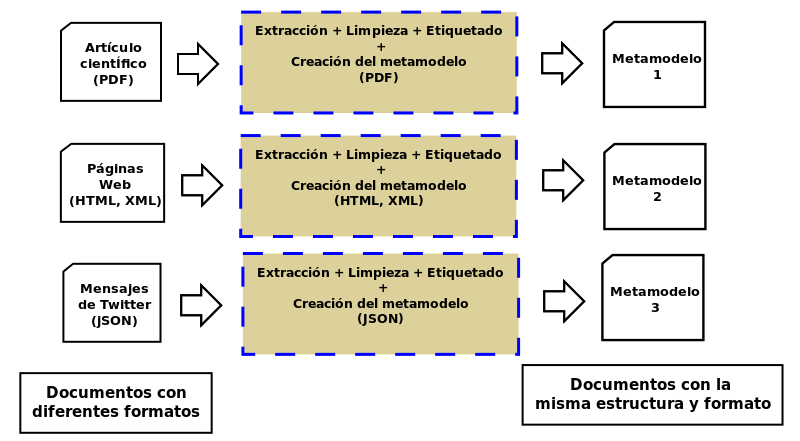
\includegraphics[width = 0.8\textwidth]{imagenes/procesoMetamodelo.png}
    \caption{Generaci\'{o}n de metamodelos para documentos de diferentes formatos}
    \label{obtencionMetamodelo}
  \end{figure}
\end{frame}


\begin{frame}
  \frametitle{Agrupamiento de metamodelos}
  En el agrupamiento se juntan los metamodelos que son muy similares entre ellos; la Figura 3 ilustra esto.

  \begin{figure}
    \centering
    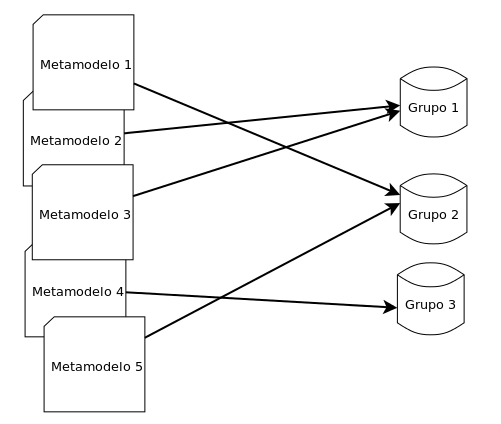
\includegraphics[width = 0.5\textwidth]{imagenes/agrupamiento.png}
    \caption{Agrupamiento de metamodelos}
    \label{agrupamientoMetamodelos}
  \end{figure}
\end{frame}

\begin{frame}
\frametitle{Agrupamiento de metamodelos}
  Se manejan dos maneras de realizar el agrupamiento:\\
  \begin{itemize}
  \item Si los metamodelos tienen asignada una de las ocho categor\'{\i}as de reporte seleccionadas, se agrupan por categor\'{\i}a.
  \vspace{2 mm}
  \item Cuando no se tiene la categor\'{\i}a del metamodelo se realiza agrupamiento no supervisado utilizando el algoritmo \textcolor{blue}{k-medias}.
  \end{itemize}
\end{frame}


\begin{frame}
  \frametitle{Entrenamiento de clasificadores}
  Para cada uno de los grupos de metamodelos se entrena un clasificador supervisado de tipo M\'{a}quina de soporte vectorial (SVM por sus siglas en ingl\'{e}s) de la siguiente manera:\\
  
  \begin{itemize}
  \item A partir de metamodelos de entrenamiento se obtiene una lista de tripletas \begin{equation}
      le = [(m_{1}^{1}, m_{2}^{1}, dup^{1}), (m_{1}^{2}, m_{2}^{2}, dup^{2}), \dots, (m_{1}^{ne}, m_{2}^{ne}, dup^{ne})],
    \end{equation} donde $m_{1}^{i}$ y $m_{2}^{i}$ son metamodelos diferentes y $dup^{i} \in [0,1]$ indica con 1 duplicado y con 0 no duplicado.
    \vspace{2 mm}
  \item Se calculan: 
    \begin{itemize}
    \item similitud de informaci\'{o}n $sinfo$
    \item similitud de lugar $slugar$
    \item diferencia de tiempo $dtiempo$ 
    \end{itemize}
  \end{itemize}
\end{frame}


\begin{frame}
  \frametitle{Entrenamiento de clasificadores}
  \begin{itemize}
  \item Se crea la matriz de caracter\'{\i}sticas $X$ y el vector de etiquetas $\vec{y}$
    \begin{equation} \label{matrizEntrenamientoClasificadores} 
      X = \begin{bmatrix}sinfo^{1},slugar^{1}, dtiempo^{1}\\
        sinfo^{2},slugar^{2}, dtiempo^{2}\\\vdots\\
        sinfo^{ne},slugar^{ne}, dtiempo^{ne}\\\end{bmatrix}
    \end{equation}
    
    \begin{equation} \label{vectorEtiquetasClasificadores}
      \vec{y} = \left[\begin{array}{c}dup^{1}\\dup^{2}\\\vdots\\dup^{ne}\end{array}\right]
    \end{equation}
    \vspace{2 mm}
  \item Finalmente se entrena el clasificador
  \end{itemize}
\end{frame}

\begin{frame}
  \frametitle{Detecci\'{o}n de duplicados}
  Los metamodelos que son agrupados se comparan contra cada uno de los metamodelos del grupo utilizando el clasificador correspondiente.\\
  \vspace{2 mm}
  Si el clasificador dicta que dos metamodelos son duplicados, entonces los reportes correspondientes son considerados duplicados. La Figura 4 ilustra la detecci\'{o}n de duplicados para dos metamodelos.

  \begin{figure}
    \centering
    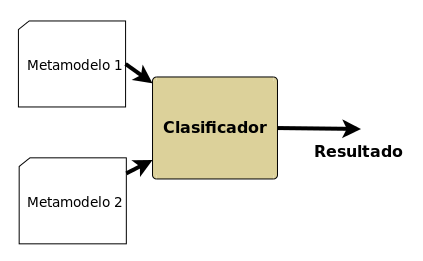
\includegraphics[width = 0.55\textwidth]{imagenes/clasificador.png}
    \caption{Detecci\'{o}n de metamodelos duplicados}
    \label{metamodelosDuplicados}
  \end{figure}
\end{frame}


\begin{frame}
  \frametitle{Resultados del etiquetador}
  Para probar el desempe\~{n}o del etiquetador se utilizaron dos archivos de 5099 palabras cada uno.\\
  \vspace{2mm}
  El contenido de un archivo fue etiquetado manualmente y para el otro archivo se utilizo el etiquetador.\\
  \vspace{2mm}
  Se compararon las etiquetas obtenidas por el etiquetador contra las etiquetas asignadas manualmente y se obtuvo una \textcolor{blue}{precisi\'{o}n} del 92\%.\\
  \vspace{2mm}
Para documentos obtenidos de Twitter esta precisi\'{o}n es muy buena y como los reportes son parecidos a los tweets, se considera un buen nivel de precisi\'{o}n obtenido por el etiquetador.
\end{frame}

\begin{frame}
  \frametitle{Resultados de la detecci\'{o}n de duplicados}
  Se prob\'{o} el desempe\~{n}o de la detecci\'{o}n de duplicados para dos enfoques diferentes:
  \vspace{2mm}
  \begin{itemize}
  \item Enfoque no supervisado o h\'{\i}brido; cuando no se conocen las categor\'{\i}as de los metamodelos durante el agrupamiento.
  \vspace{2mm}
  \item Enfoque supervisado; cuando se conocen las categor\'{\i}as de los metamodelos durante el agrupamiento. 
  \end{itemize}

\end{frame}

\begin{frame}
  \frametitle{Resultados de la detecci\'{o}n de duplicados}
  Para el enfoque h\'{\i}brido se obtuvo un valor promedio de \textcolor{blue}{precisi\'{o}n} del 46.9\% y para el enfoque supervisado del 54.5\%.\\
  
  \begin{figure}
    \centering
    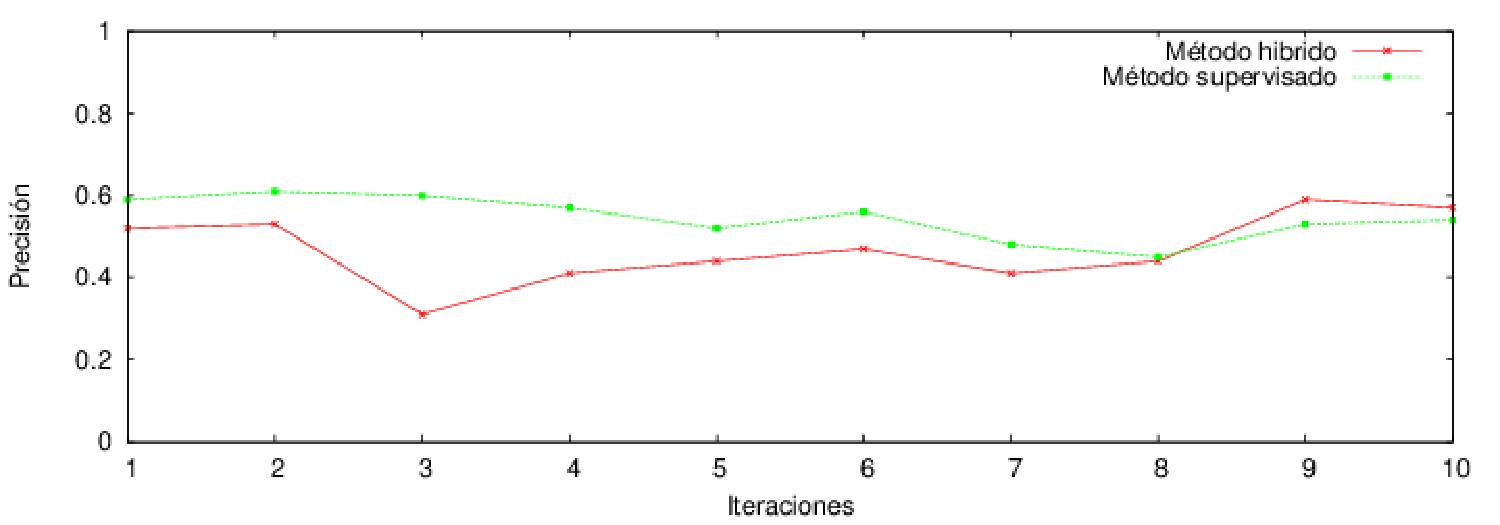
\includegraphics[width = 1.0\textwidth]{imagenes/precisioni3.pdf}
    \caption{Valores de precisi\'{o}n obtenidos en la detecci\'{o}n de duplicados}
    \label{resultadoPrecision}
  \end{figure}
\end{frame}

\begin{frame}
  \frametitle{Resultados de la detecci\'{o}n de duplicados}
  Para el enfoque h\'{\i}brido se obtuvo un valor promedio del \textcolor{blue}{valor-F} del 59.6\% y para el enfoque supervisado del 65.6\%.\\

  \begin{figure}
    \centering
    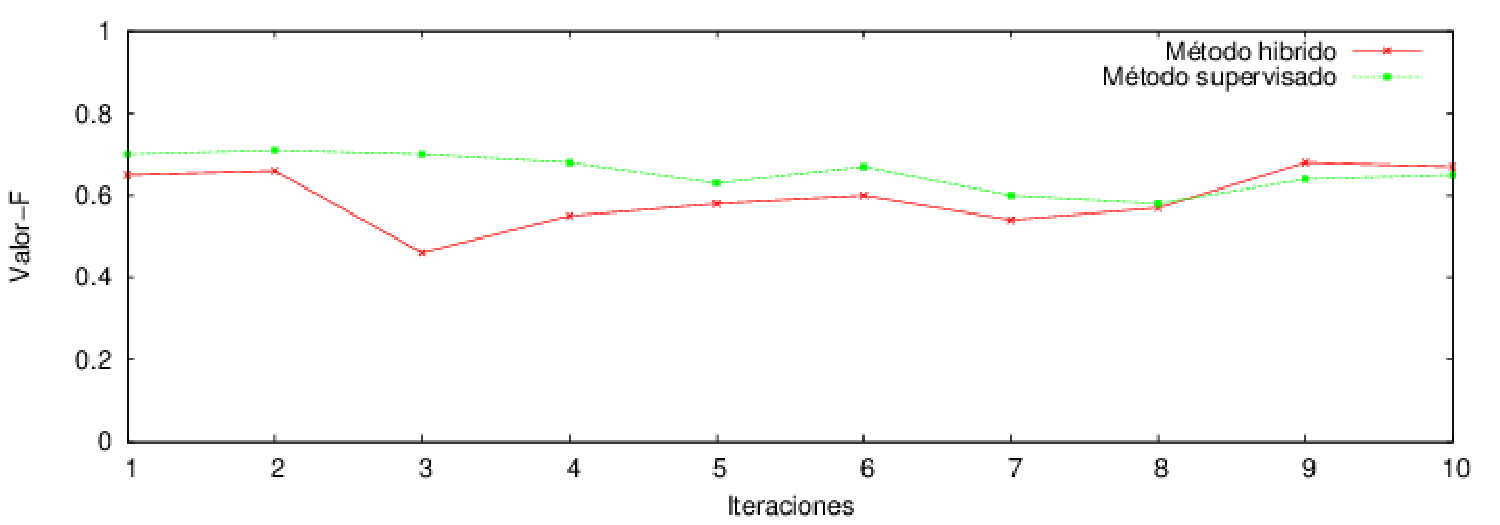
\includegraphics[width = 1.0\textwidth]{imagenes/fmeasurei3.pdf}
    \caption{Valores F obtenidos en la detecci\'{o}n de duplicados}
    \label{resultadoValorF}
  \end{figure}
\end{frame}

\begin{frame}
  \frametitle{Resultados de la detecci\'{o}n de duplicados}
   Los resultados obtenidos muestran que el m\'{e}todo supervisado tiene un mejor desempe\~{n}o que el m\'{e}todo h\'{\i}brido.\\ 
   \vspace{2mm}
Sin embargo, hay que observar el contenido los grupos resultantes del agrupamiento del m\'{e}todo h\'{\i}brido, porque estos pueden mostrar nuevas relaciones entre los reportes.\\
   \vspace{2mm}
   Para el tipo de documentos con los que se trabaja, los resultados son obtenidos parecen ser favorables.
\end{frame}


\begin{frame}
  \frametitle{Trabajos relacionados}
  \begin{itemize}
  \item Agarwal, Vaithiyanathan, Sharma, and GautamShroff 2012. Detectan noticias locales reportadas en Twitter, correspondientes a ``huelgas de trabajo'' y ``incendios en f\'{a}bricas.''\\
    \vspace{2mm}
  \item Broder 2000. Detecta documentos duplicados agrupando representaciones creadas a partir de n-gramas.\\
    \vspace{2mm}
  \item Sankaranarayanan, Samet, Teitler, Lieberman, and Sperling 2009. Implementan un sistema de generaci\'{o}n de noticias a partir de mensajes en Twitter.\\
    \vspace{2mm}
  \item Tao, Abel, Hauff, Houben, and Gadiraju 2013. Presentan un m\'{e}todo de detecci\'{o}n de duplicados para mensajes de Twitter.
  \end{itemize}
\end{frame}

\begin{frame}
  \frametitle{Estado actual de la tesis}
  \begin{itemize}
  \item Por ahora se est\'{a} corrigiendo los cap\'{\i}tulos de la tesis que ya fueron escritos.
    \vspace{2mm}
  \item Todos los experimentos ya fueron realizados.
    \vspace{2mm}
  \item Falta por escribir los cap\'{\i}tulos de: introducci\'{o}n, resumen y conclusi\'{o}n.
  \end{itemize}
\end{frame}

\end{document}
